%% generato automaticamente da tools/build_tex.py --- non modificare
\chapter{Le funzioni iperboliche di $\pi$ ed $\mathrm{e}$}
\label{cap:sin-cos}
\quaderno{sin-cos.dfw}{04 Jan 2010}{20}

Gennaio 2010. Venti espressioni che costruiscono, pezzo per pezzo, un sistema completo di funzioni iperboliche e circolari a partire da due sole basi: $\mathrm{e}^{\pi x}$ e $\pi^{\mathrm{e}x}$. È il quaderno tecnicamente più compatto della raccolta, perché tutto quello che contiene discende da una sola osservazione, che però non è mai scritta esplicitamente.

\section{Il sistema iperbolico}

L'osservazione da cui dipende tutto è questa: $\dfrac{\mathrm{e}^{\pi x}}{\pi^{\mathrm{e}x}}=\mathrm{e}^{\pi x-\mathrm{e}x\ln\pi}=\mathrm{e}^{kx}$, dove $k=\pi-\mathrm{e}\ln\pi$. Il rapporto fra le due potenze è dunque un semplice esponenziale, e la costante $k$ ne è la pulsazione. Da qui le prime quattro espressioni si leggono a colpo d'occhio.

\begin{espr}{1}{User}{}
\[
\frac{\frac{\mathrm{e}^{\pi\, x}}{\pi^{\mathrm{e}\, x}} + \frac{\pi^{\mathrm{e}\, x}}{\mathrm{e}^{\pi\, x}}}{2}
\]
\end{espr}
La semisomma del rapporto e del suo reciproco: è $\cosh(kx)$ con $k=\pi-\mathrm{e}\ln\pi$.

\begin{espr}{2}{User}{}
\[
\frac{\frac{\mathrm{e}^{\pi\, x}}{\pi^{\mathrm{e}\, x}} - \frac{\pi^{\mathrm{e}\, x}}{\mathrm{e}^{\pi\, x}}}{2}
\]
\end{espr}
La semidifferenza: $\sinh(kx)$.

\begin{espr}{3}{User}{}
\[
\frac{\mathrm{e}^{2\, \pi\, x} - \pi^{2\, \mathrm{e}\, x}}{\pi^{2\, \mathrm{e}\, x} + \mathrm{e}^{2\, \pi\, x}}
\]
\end{espr}
Il loro rapporto, cioè $\tanh(kx)$. Gli esponenti raddoppiati vengono dal prodotto delle due espressioni precedenti.

\begin{espr}{4}{User}{}
\[
\frac{\pi^{2\, \mathrm{e}\, x} + \mathrm{e}^{2\, \pi\, x}}{\mathrm{e}^{2\, \pi\, x} - \pi^{2\, \mathrm{e}\, x}}
\]
\end{espr}
Il reciproco: $\coth(kx)$.


Sono, nell'ordine, $\cosh(kx)$, $\sinh(kx)$, $\tanh(kx)$ e $\coth(kx)$. Le definizioni sono quelle canoniche — semisomma, semidifferenza, loro rapporto — solo scritte con basi inconsuete.

\section{Le derivate}

Le quattro espressioni successive sono le derivate delle precedenti, e confermano che il sistema è coerente: la costante $k$ compare come fattore, esattamente come ci si aspetta derivando una funzione di $kx$.

\begin{espr}{5}{User}{}
\[
\left(\pi - \mathrm{e}\, \ln\!\left(\pi\right)\right)\, \left(\frac{\frac{\mathrm{e}^{\pi\, x}}{\pi^{\mathrm{e}\, x}} - \frac{\pi^{\mathrm{e}\, x}}{\mathrm{e}^{\pi\, x}}}{2}\right)
\]
\end{espr}
$k\sinh(kx)$: la derivata del coseno iperbolico.

\begin{espr}{6}{User}{}
\[
\left(\pi - \mathrm{e}\, \ln\!\left(\pi\right)\right)\, \left(\frac{\frac{\mathrm{e}^{\pi\, x}}{\pi^{\mathrm{e}\, x}} + \frac{\pi^{\mathrm{e}\, x}}{\mathrm{e}^{\pi\, x}}}{2}\right)
\]
\end{espr}
$k\cosh(kx)$: la derivata del seno iperbolico.

\begin{espr}{7}{User}{}
\[
\frac{4\, \pi^{2\, \mathrm{e}\, x}\, \mathrm{e}^{2\, \pi\, x}\, \left(\pi - \mathrm{e}\, \ln\!\left(\pi\right)\right)}{\left(\mathrm{e}^{2\, \pi\, x} + \pi^{2\, \mathrm{e}\, x}\right)^{2}}
\]
\end{espr}
$k\,\mathrm{sech}^2(kx)$: la derivata della tangente iperbolica.

\begin{espr}{8}{User}{}
\[
\frac{4\, \pi^{2\, \mathrm{e}\, x}\, \mathrm{e}^{2\, \pi\, x}\, \left(\mathrm{e}\, \ln\!\left(\pi\right) - \pi\right)}{\left(\mathrm{e}^{2\, \pi\, x} - \pi^{2\, \mathrm{e}\, x}\right)^{2}}
\]
\end{espr}
$-k\,\mathrm{csch}^2(kx)$: la derivata della cotangente iperbolica. Il fattore $(\mathrm{e}\ln\pi-\pi)$ è $-k$.


In particolare $\#7$, che sembra un'espressione complicata, è $k\,\mathrm{sech}^2(kx)$: dividendo numeratore e denominatore per $\pi^{4\mathrm{e}x}$ resta $4k\,\mathrm{e}^{2kx}/\left(\mathrm{e}^{2kx}+1\right)^2$, che è la derivata della tangente iperbolica. L'espressione $\#8$ è invece $-k\,\mathrm{csch}^2(kx)$, la derivata della cotangente iperbolica.

\section{Il passaggio al caso circolare}

Sostituendo $x$ con $\mathrm{i}x$ le funzioni iperboliche diventano circolari. Le sei espressioni che seguono lo verificano e ne traggono la formula di addizione.

\begin{espr}{9}{User}{}
\begin{align*}
& \frac{\frac{\mathrm{e}^{\pi\, \left(\mathrm{i}\, x\right)}}{\pi^{\mathrm{e}\, \left(\mathrm{i}\, x\right)}} + \frac{\pi^{\mathrm{e}\, \left(\mathrm{i}\, x\right)}}{\mathrm{e}^{\pi\, \left(\mathrm{i}\, x\right)}}}{2} \\
=\;& \cos\!\left(\pi\, x\right)\, \cos\!\left(\mathrm{e}\, x\, \ln\!\left(\pi\right)\right) + \sin\!\left(\pi\, x\right)\, \sin\!\left(\mathrm{e}\, x\, \ln\!\left(\pi\right)\right) = \cos\!\left(\left(\pi - \mathrm{e}\, \ln\!\left(\pi\right)\right)\, x\right)
\end{align*}
\end{espr}
Sostituendo $x\to\mathrm{i}x$ il coseno iperbolico diventa circolare, e la scrittura esplicita è la formula di sottrazione del coseno.

\begin{espr}{10}{User}{\verificata}
\begin{align*}
& \frac{\frac{\mathrm{e}^{\pi\, \left(\mathrm{i}\, x\right)}}{\pi^{\mathrm{e}\, \left(\mathrm{i}\, x\right)}} - \frac{\pi^{\mathrm{e}\, \left(\mathrm{i}\, x\right)}}{\mathrm{e}^{\pi\, \left(\mathrm{i}\, x\right)}}}{2} \\
=\;& \mathrm{i}\, \left(\sin\!\left(\pi\, x\right)\, \cos\!\left(\mathrm{e}\, x\, \ln\!\left(\pi\right)\right) - \cos\!\left(\pi\, x\right)\, \sin\!\left(\mathrm{e}\, x\, \ln\!\left(\pi\right)\right)\right) \\
=\;& \mathrm{i}\, \sin\!\left(\left(\pi - \mathrm{e}\, \ln\!\left(\pi\right)\right)\, x\right)
\end{align*}
\end{espr}
Analogamente per il seno: il fattore $\mathrm{i}$ segnala che $\sinh(\mathrm{i}\theta)=\mathrm{i}\sin\theta$.

\begin{espr}{11}{User}{\verificata}
\begin{align*}
& \frac{\frac{\mathrm{e}^{\pi\, \left(\mathrm{i}\, x\right)}}{\pi^{\mathrm{e}\, \left(\mathrm{i}\, x\right)}} + \frac{\pi^{\mathrm{e}\, \left(\mathrm{i}\, x\right)}}{\mathrm{e}^{\pi\, \left(\mathrm{i}\, x\right)}}}{2} \\
&\qquad + \frac{\frac{\mathrm{e}^{\pi\, \left(\mathrm{i}\, x\right)}}{\pi^{\mathrm{e}\, \left(\mathrm{i}\, x\right)}} - \frac{\pi^{\mathrm{e}\, \left(\mathrm{i}\, x\right)}}{\mathrm{e}^{\pi\, \left(\mathrm{i}\, x\right)}}}{2} \\
=\;& \mathrm{e}^{\mathrm{i}\, x\, \left(\pi - \mathrm{e}\, \ln\!\left(\pi\right)\right)}
\end{align*}
\end{espr}
La somma delle due ricompone l'esponenziale complesso di pulsazione $k$.

\begin{espr}{12}{User}{\verificata}
\begin{align*}
& \frac{\frac{\mathrm{e}^{\pi\, \left(\mathrm{i}\, x\right)}}{\pi^{\mathrm{e}\, \left(\mathrm{i}\, x\right)}} + \frac{\pi^{\mathrm{e}\, \left(\mathrm{i}\, x\right)}}{\mathrm{e}^{\pi\, \left(\mathrm{i}\, x\right)}}}{2} \\
&\qquad - \frac{\frac{\mathrm{e}^{\pi\, \left(\mathrm{i}\, x\right)}}{\pi^{\mathrm{e}\, \left(\mathrm{i}\, x\right)}} - \frac{\pi^{\mathrm{e}\, \left(\mathrm{i}\, x\right)}}{\mathrm{e}^{\pi\, \left(\mathrm{i}\, x\right)}}}{2} \\
=\;& \mathrm{e}^{-\mathrm{i}\, x\, \left(\pi - \mathrm{e}\, \ln\!\left(\pi\right)\right)}
\end{align*}
\end{espr}
La differenza dà l'esponenziale coniugato.

\begin{espr}{13}{User}{\verificata}
\begin{align*}
& \frac{\frac{\mathrm{e}^{\pi\, \left(\mathrm{i}\, x\right)}}{\pi^{\mathrm{e}\, \left(\mathrm{i}\, x\right)}} + \frac{\pi^{\mathrm{e}\, \left(\mathrm{i}\, x\right)}}{\mathrm{e}^{\pi\, \left(\mathrm{i}\, x\right)}}}{2} \\
&\qquad + \frac{\mathrm{i}\, \left(\frac{\mathrm{e}^{\pi\, \left(\mathrm{i}\, x\right)}}{\pi^{\mathrm{e}\, \left(\mathrm{i}\, x\right)}} - \frac{\pi^{\mathrm{e}\, \left(\mathrm{i}\, x\right)}}{\mathrm{e}^{\pi\, \left(\mathrm{i}\, x\right)}}\right)}{2} \\
=\;& \cos\!\left(\left(\pi - \mathrm{e}\, \ln\!\left(\pi\right)\right)\, x\right) - \sin\!\left(\left(\pi - \mathrm{e}\, \ln\!\left(\pi\right)\right)\, x\right)
\end{align*}
\end{espr}
Una combinazione con il fattore $\mathrm{i}$: il risultato è $\cos-\sin$.

\begin{espr}{14}{User}{\verificata}
\begin{align*}
& \frac{\frac{\mathrm{e}^{\pi\, \left(\mathrm{i}\, x\right)}}{\pi^{\mathrm{e}\, \left(\mathrm{i}\, x\right)}} + \frac{\pi^{\mathrm{e}\, \left(\mathrm{i}\, x\right)}}{\mathrm{e}^{\pi\, \left(\mathrm{i}\, x\right)}}}{2} \\
&\qquad - \frac{\mathrm{i}\, \left(\frac{\mathrm{e}^{\pi\, \left(\mathrm{i}\, x\right)}}{\pi^{\mathrm{e}\, \left(\mathrm{i}\, x\right)}} - \frac{\pi^{\mathrm{e}\, \left(\mathrm{i}\, x\right)}}{\mathrm{e}^{\pi\, \left(\mathrm{i}\, x\right)}}\right)}{2} \\
=\;& \cos\!\left(\left(\pi - \mathrm{e}\, \ln\!\left(\pi\right)\right)\, x\right) + \sin\!\left(\left(\pi - \mathrm{e}\, \ln\!\left(\pi\right)\right)\, x\right)
\end{align*}
\end{espr}
L'altra combinazione: $\cos+\sin$.


La riga $\#9$ contiene la formula di sottrazione del coseno: $\cos(\pi x)\cos(\mathrm{e}x\ln\pi)+\sin(\pi x)\sin(\mathrm{e}x\ln\pi)=\cos\!\big((\pi-\mathrm{e}\ln\pi)x\big)$. Le due frequenze $\pi$ ed $\mathrm{e}\ln\pi$ sono quasi uguali, e la loro differenza è la piccolissima $k$: è il fenomeno del battimento, due oscillazioni rapide e vicine che si combinano in una lentissima. Le righe $\#11$ e $\#12$ ricompongono l'esponenziale complesso, e le ultime due danno le combinazioni $\cos\mp\sin$.

\section{Quanto vale $k$}

L'ultima sezione mette i numeri. Sono sei righe, e insieme dicono una cosa sola con precisione notevole.

\begin{espr}{15}{User}{\verificata}
\[
\pi - \mathrm{e}\, \ln\!\left(\pi\right) = 0.02989420638
\]
\end{espr}
Il valore numerico della costante: circa tre centesimi.

\begin{espr}{16}{User}{\verificata}
\[
\frac{\pi^{-\mathrm{e}}\, \mathrm{e}^{\pi}}{2} - \frac{\pi^{\mathrm{e}}\, \mathrm{e}^{-\pi}}{2} = 0.02989865914
\]
\end{espr}
Il seno iperbolico di $k$, calcolato dalla definizione. Notare che $\pi^{-\mathrm{e}}\mathrm{e}^{\pi}=\mathrm{e}^{k}$.

\begin{espr}{17}{User}{}
\begin{align*}
& \pi - \mathrm{e}\, \ln\!\left(\pi\right) \\
=\;& \frac{\frac{\mathrm{e}^{\pi\, x}}{\pi^{\mathrm{e}\, x}} - \frac{\pi^{\mathrm{e}\, x}}{\mathrm{e}^{\pi\, x}}}{2}
\end{align*}
\end{espr}
L'equazione $\sinh(kx)=k$: si chiede per quale $x$ il seno iperbolico restituisca l'argomento.

\begin{espr}{18}{User}{}
\begin{align*}
& x \\
=\;& \frac{\ln\!\left(\sqrt{\mathrm{e}^{2}\, \ln^{2}\!\left(\pi\right) - 2\, \pi\, \mathrm{e}\, \ln\!\left(\pi\right) + \pi^{2} + 1} - \mathrm{e}\, \ln\!\left(\pi\right) + \pi\right)}{\pi - \mathrm{e}\, \ln\!\left(\pi\right)} \\
=\;& 0.9998511159
\end{align*}
\end{espr}
La soluzione è $\operatorname{arcsinh}(k)/k$, cioè $0{,}99985$: non uno, e la distanza da uno misura la non linearità del seno iperbolico.

\begin{espr}{19}{User}{\verificata}
\[
\frac{\pi^{\mathrm{e}}\, \mathrm{e}^{-\pi}}{2} + \frac{\pi^{-\mathrm{e}}\, \mathrm{e}^{\pi}}{2} = 1.000446865
\]
\end{espr}
Il coseno iperbolico di $k$: eccede l'unità di circa $k^2/2=4{,}47\cdot10^{-4}$.

\begin{espr}{20}{User}{\verificata}
\begin{align*}
& \frac{\pi^{-\mathrm{e}}\, \mathrm{e}^{\pi}}{2} - \frac{\pi^{\mathrm{e}}\, \mathrm{e}^{-\pi}}{2} - \pi + \mathrm{e}\, \ln\!\left(\pi\right) \\
=\;& 4.452759521 \cdot 10^{-6}
\end{align*}
\end{espr}
Lo scarto $\sinh k-k$, che vale $k^3/6$. È il termine di terzo grado dello sviluppo in serie, isolato numericamente.

\begin{figure}[htbp]
  \centering
  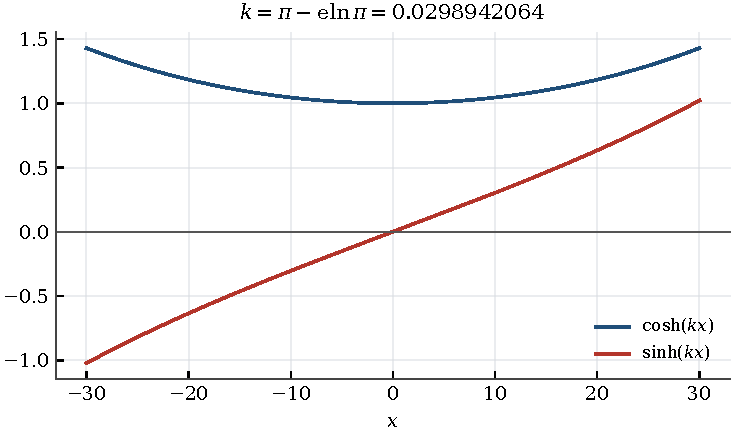
\includegraphics[width=0.86\linewidth]{../figures/sincos_pi_e.pdf}
  \caption{Le funzioni $\cosh(kx)$ e $\sinh(kx)$ costruite nel quaderno. La pulsazione $k=\pi-\mathrm{e}\ln\pi$ è così piccola che occorre arrivare a $|x|\approx 30$ per vederle crescere.}
  \label{fig:sincos_pi_e}
\end{figure}

Ecco il conto. La costante vale $k=\pi-\mathrm{e}\ln\pi=0{,}02989420\ldots$, un numero molto piccolo. La riga $\#16$ calcola $\sinh k=0{,}02989865\ldots$ e la riga $\#19$ calcola $\cosh k=1{,}000446865$. Per $k$ così piccolo si ha $\sinh k\approx k$ e $\cosh k\approx 1$, e le due righe lo confermano.

Ma il quaderno non si accontenta e chiede di quanto esattamente $\sinh k$ superi $k$: è la riga $\#20$, che dà $4{,}4527\cdot10^{-6}$. Questo numero è $k^3/6$, cioè il primo termine trascurato nello sviluppo $\sinh k=k+\tfrac{k^3}{3!}+\cdots$ — e infatti $0{,}0298942^3/6=4{,}4528\cdot10^{-6}$. Le sei righe finali sono, in sostanza, una verifica numerica dello sviluppo in serie del seno iperbolico, condotta su un argomento scelto in modo che il primo termine correttivo fosse misurabile.

La riga $\#18$ chiude con eleganza: risolvendo $\sinh(kx)=k$ si trova $x=\operatorname{arcsinh}(k)/k=0{,}9998511$. Il valore $x=1$ non è soluzione proprio perché $\sinh k\neq k$, e lo scarto dall'unità, un centocinquantamillesimo, è la misura di quella differenza.

\section*{In sintesi}
\addcontentsline{toc}{section}{In sintesi}

Il quaderno è costruito su una sola identità elementare — il rapporto fra $\mathrm{e}^{\pi x}$ e $\pi^{\mathrm{e}x}$ è $\mathrm{e}^{kx}$ — e su una sola osservazione numerica: quel $k$ è molto piccolo. Da lì discendono un sistema iperbolico completo con le sue derivate, il corrispondente sistema circolare, e una misura sperimentale del terzo termine dello sviluppo del seno iperbolico. Il numero $\sinh k=0{,}0298986\ldots$ che compare alla riga $\#16$ ricomparirà, sette mesi dopo, alla riga $\#69$ di \dfw{e.dfw} (capitolo~\ref{cap:e}), calcolato per un'altra strada e senza che il legame venga notato.

